\chapter{Appendix}
\label{appendix}


\begin{figure}[h]
\begin{center}
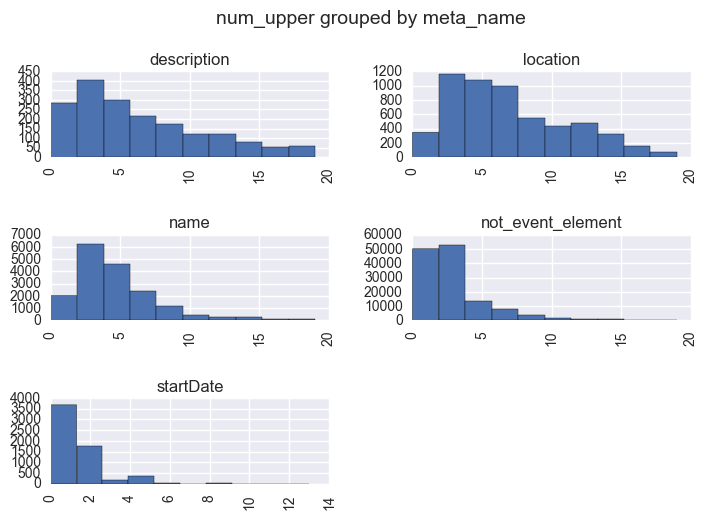
\includegraphics[width=1.0\textwidth]{figures/distrUpperByMeta}
\caption{Distribution of upper case letters number by meta name}
\label{fig:distrUpperByMeta}
\end{center}
\end{figure}

\begin{figure}[h]
\begin{center}
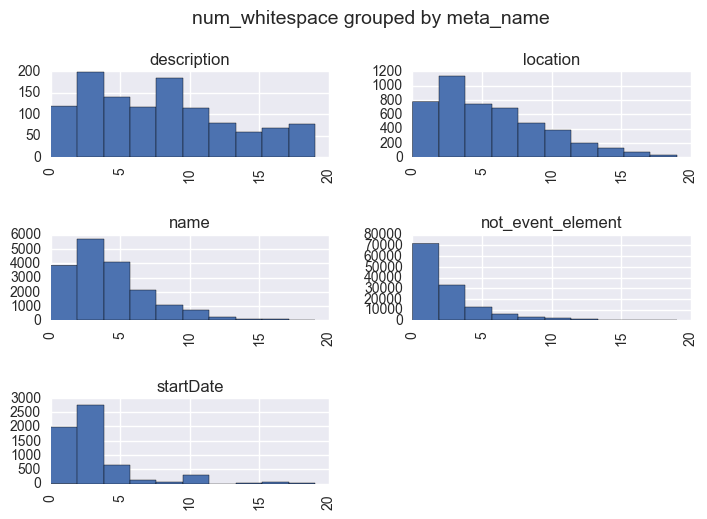
\includegraphics[width=1.0\textwidth]{figures/distrWhiteByMeta}
\caption{Distribution of white spaces by meta name}
\label{fig:distrWhiteByMeta}
\end{center}
\end{figure}

\begin{figure}[h]
\begin{center}
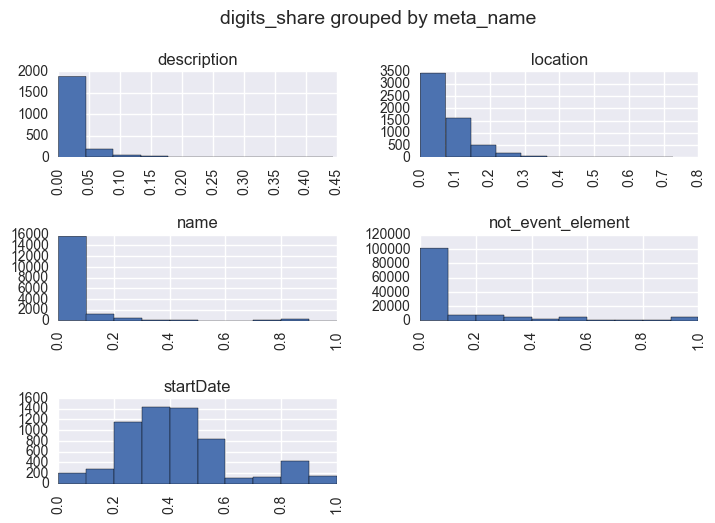
\includegraphics[width=1.0\textwidth]{figures/distrDigitPropByMeta}
\caption{Distribution of digit proportion by meta name}
\label{fig:distrDigitPropByMeta}
\end{center}
\end{figure}

\begin{figure}[h]
\begin{center}
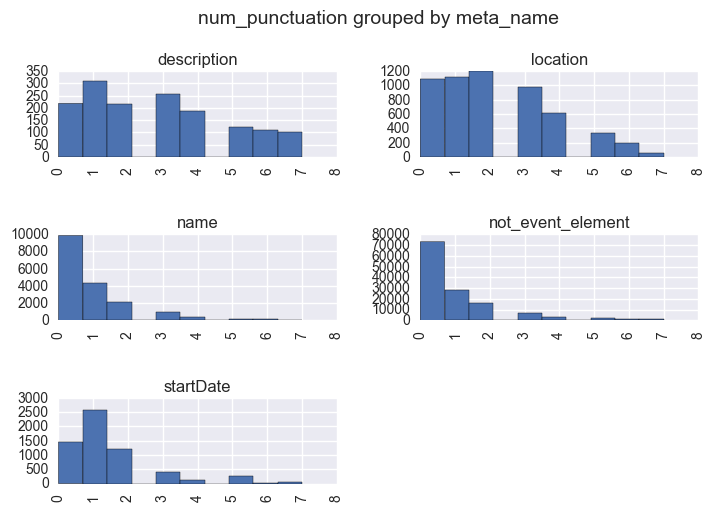
\includegraphics[width=1.0\textwidth]{figures/distrPunctByMeta}
\caption{Distribution of punctuation marks number by meta name}
\label{fig:distrPunctByMeta}
\end{center}
\end{figure}

\begin{table}[h]
\begin{center}

\begin{tabular}{llrrrrrr}
\toprule
            &       &  digit\_share &  num\_digit &   num\_punc &    num\_upp &  num\_white &   text\_len \\
meta\_name & {} &              &            &            &            &            &            \\
\midrule
description & count &      2206.00 &    2206.00 &    2206.00 &    2206.00 &    2206.00 &    2206.00 \\
            & mean &         0.02 &       1.99 &       2.23 &       5.70 &       5.41 &      43.14 \\
            & std &         0.05 &       3.28 &       1.94 &       4.59 &       4.72 &      32.55 \\
            & min &         0.00 &       0.00 &       0.00 &       0.00 &       0.00 &       1.00 \\
            & 25\% &         0.00 &       0.00 &       0.96 &       3.00 &       2.65 &      23.02 \\
            & 50\% &         0.00 &       0.00 &       1.00 &       4.00 &       2.65 &      23.02 \\
            & 75\% &         0.02 &       2.00 &       3.00 &       8.00 &       8.00 &      60.00 \\
            & max &         0.44 &      14.00 &       7.00 &      19.00 &      19.00 &     141.00 \\
location & count &      5780.00 &    5780.00 &    5780.00 &    5780.00 &    5780.00 &    5780.00 \\
            & mean &         0.06 &       3.27 &       2.12 &       6.74 &       4.87 &      47.45 \\
            & std &         0.08 &       3.65 &       1.69 &       4.35 &       3.85 &      30.90 \\
            & min &         0.00 &       0.00 &       0.00 &       0.00 &       0.00 &       1.00 \\
            & 25\% &         0.00 &       0.00 &       1.00 &       3.00 &       2.65 &      23.00 \\
            & 50\% &         0.04 &       1.62 &       2.00 &       6.00 &       3.00 &      42.00 \\
            & 75\% &         0.11 &       6.00 &       3.00 &      10.00 &       7.00 &      69.00 \\
            & max &         0.73 &      14.00 &       7.00 &      19.00 &      19.00 &     141.00 \\
name & count &     18116.00 &   18116.00 &   18116.00 &   18116.00 &   18116.00 &   18116.00 \\
            & mean &         0.05 &       1.07 &       0.85 &       4.46 &       3.97 &      32.32 \\
            & std &         0.14 &       2.41 &       1.25 &       3.25 &       3.11 &      20.12 \\
            & min &         0.00 &       0.00 &       0.00 &       0.00 &       0.00 &       2.00 \\
            & 25\% &         0.00 &       0.00 &       0.00 &       2.00 &       2.00 &      18.00 \\
            & 50\% &         0.00 &       0.00 &       0.00 &       4.00 &       3.00 &      27.00 \\
            & 75\% &         0.00 &       0.00 &       1.00 &       6.00 &       5.00 &      42.00 \\
            & max &         1.00 &      14.00 &       7.00 &      19.00 &      19.00 &     141.00 \\
not\_event & count &    135665.00 &  135665.00 &  135665.00 &  135665.00 &  135665.00 &  135665.00 \\
            & mean &         0.11 &       1.43 &       0.88 &       2.70 &       2.33 &      20.70 \\
            & std &         0.23 &       2.60 &       1.31 &       2.83 &       3.08 &      21.49 \\
            & min &         0.00 &       0.00 &       0.00 &       0.00 &       0.00 &       1.00 \\
            & 25\% &         0.00 &       0.00 &       0.00 &       1.00 &       0.00 &       8.00 \\
            & 50\% &         0.00 &       0.00 &       0.00 &       2.00 &       1.00 &      14.00 \\
            & 75\% &         0.10 &       2.00 &       1.00 &       3.00 &       3.00 &      24.00 \\
            & max &         1.00 &      14.00 &       7.00 &      19.00 &      19.00 &     141.00 \\
startDate & count &      6105.00 &    6105.00 &    6105.00 &    6105.00 &    6105.00 &    6105.00 \\
            & mean &         0.41 &       5.74 &       1.40 &       1.38 &       2.75 &      16.54 \\
            & std &         0.20 &       3.01 &       1.36 &       1.36 &       2.92 &      10.98 \\
            & min &         0.00 &       0.00 &       0.00 &       0.00 &       0.00 &       1.00 \\
            & 25\% &         0.29 &       3.00 &       1.00 &       0.00 &       1.00 &       9.00 \\
            & 50\% &         0.39 &       6.00 &       1.00 &       1.00 &       2.00 &      14.00 \\
            & 75\% &         0.50 &       8.00 &       2.00 &       2.00 &       3.00 &      22.00 \\
            & max &         1.00 &      14.00 &       7.00 &      13.00 &      19.00 &     122.00 \\
\bottomrule
\end{tabular}

\caption{Summary statistics for a textual features grouped by meta name}
\label{table:textualDistr}
\end{center}
\end{table}      



\begin{table}
\begin{center}


\begin{tabular}{llrr}
\toprule
            &       &   x\_center &   y\_center \\
meta\_name & {} &            &            \\
\midrule
description & count &    2206.00 &    2206.00 \\
            & mean &     262.80 &    3112.37 \\
            & std &     135.67 &    2599.73 \\
            & min &      23.50 &     120.50 \\
            & 25\% &     200.00 &     805.62 \\
            & 50\% &     200.00 &    2247.50 \\
            & 75\% &     279.75 &    6151.55 \\
            & max &     920.50 &   13226.00 \\
location & count &    5780.00 &    5780.00 \\
            & mean &     283.90 &    2017.20 \\
            & std &     192.64 &    2072.98 \\
            & min &      35.50 &     120.50 \\
            & 25\% &     189.50 &     602.00 \\
            & 50\% &     200.00 &    1210.50 \\
            & 75\% &     312.12 &    2635.12 \\
            & max &     900.00 &   13168.50 \\
name & count &   18116.00 &   18116.00 \\
            & mean &     248.27 &    2157.42 \\
            & std &     152.47 &    2354.20 \\
            & min &      14.50 &      27.00 \\
            & 25\% &     167.00 &     479.50 \\
            & 50\% &     200.00 &    1163.00 \\
            & 75\% &     284.50 &    3010.62 \\
            & max &     920.50 &   13248.50 \\
not\_event\_element & count &  135665.00 &  135665.00 \\
            & mean &     305.94 &    7076.33 \\
            & std &     210.60 &   10007.35 \\
            & min &       0.00 &       4.50 \\
            & 25\% &     153.50 &    1397.00 \\
            & 50\% &     235.00 &    3060.50 \\
            & 75\% &     419.00 &    6957.50 \\
            & max &    1418.00 &   53955.00 \\
startDate & count &    6105.00 &    6105.00 \\
            & mean &     180.83 &    2465.70 \\
            & std &     145.79 &    2326.51 \\
            & min &      19.00 &      34.50 \\
            & 25\% &      89.00 &     676.00 \\
            & 50\% &     137.50 &    1570.50 \\
            & 75\% &     203.50 &    3540.50 \\
            & max &     887.50 &   13239.50 \\
\bottomrule
\end{tabular}

\caption{Summary statistics for a spatial features grouped by meta name}
\label{table:spatialDistr}
\end{center}
\end{table}  


\begin{figure}[h]
\begin{center}
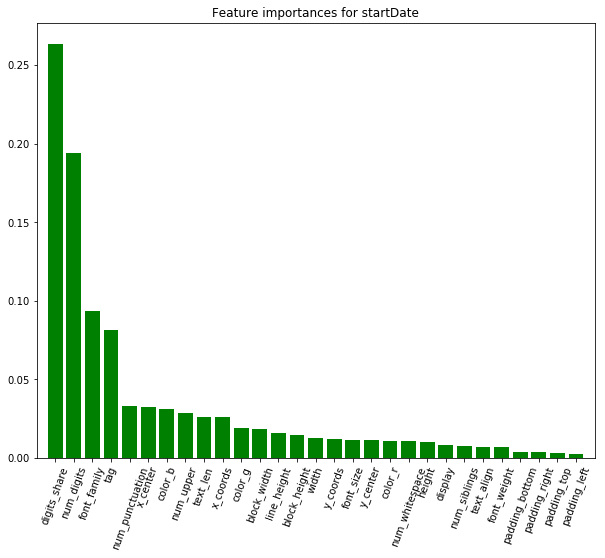
\includegraphics[width=1.0\textwidth]{figures08/importanceDate}
\caption{Feature importance from Random Forest for the Event date, Top: digits share, number of digits, font family, tag, number of punctuation}
\label{fig:importanceDate}
\end{center}
\end{figure}

\begin{figure}[h]
\begin{center}
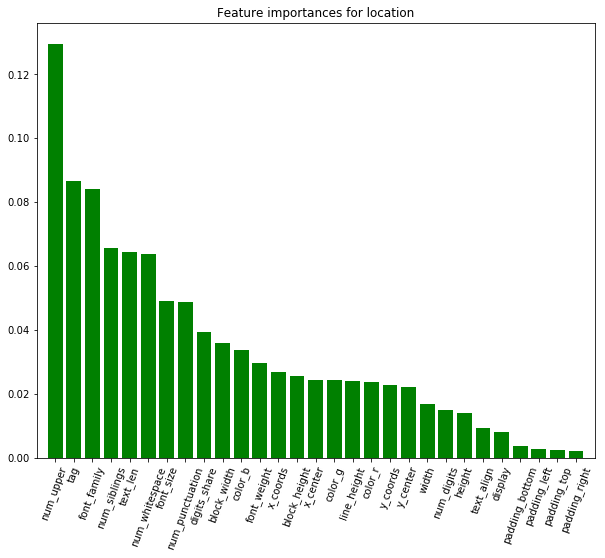
\includegraphics[width=1.0\textwidth]{figures08/importanceLocation}
\caption{Feature importance from Random Forest for the Event location, Top: number of uppercase letters, tag, font family, number of siblings, text length}
\label{fig:importanceLocation}
\end{center}
\end{figure}

\begin{figure}[h]
\begin{center}
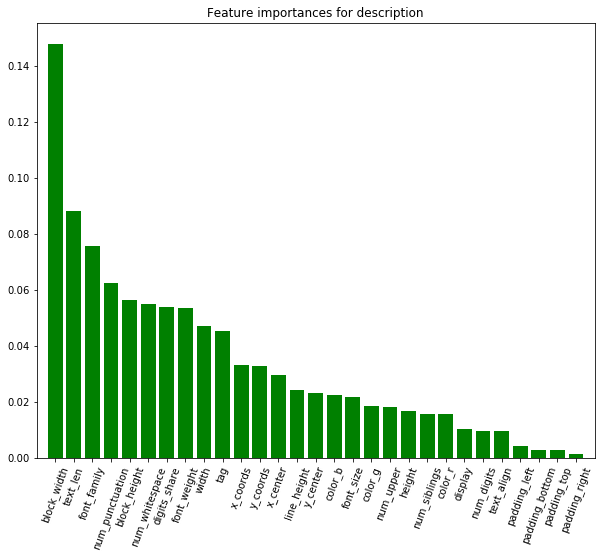
\includegraphics[width=1.0\textwidth]{figures08/importanceDescription}
\caption{Feature importance from Random Forest for the Event description, Top: block width, text length, font family, number of punctuation}
\label{fig:importanceDescription}
\end{center}
\end{figure}


\begin{table}[h]
\begin{center}
{\renewcommand{\arraystretch}{1.2}
\begin{tabular}{lrrrrll}
\toprule
accuracy &    f1 &  precision &  recall &    meta\_name &                  model \\
\midrule
0.98 &  0.98 &       0.98 &    0.97 &         name &          Random forest \\
0.58 &  0.70 &       0.54 &    1.00 &         name &                    SVM \\
0.82 &  0.82 &       0.81 &    0.82 &         name &    Logistic regression \\
0.98 &  0.98 &       0.98 &    0.97 &         name &  Extreme Random Forest \\
\midrule
0.97 &  0.97 &       0.97 &    0.96 &     location &          Random forest \\
0.59 &  0.71 &       0.56 &    1.00 &     location &                    SVM \\
0.82 &  0.82 &       0.81 &    0.84 &     location &    Logistic regression \\
0.97 &  0.97 &       0.97 &    0.97 &     location &  Extreme Random Forest \\
\midrule
0.95 &  0.95 &       0.96 &    0.94 &  description &          Random forest \\
0.51 &  0.66 &       0.50 &    1.00 &  description &                    SVM \\
0.87 &  0.88 &       0.87 &    0.88 &  description &    Logistic regression \\
0.96 &  0.96 &       0.98 &    0.95 &  description &  Extreme Random Forest \\
\midrule
0.98 &  0.98 &       0.97 &    0.99 &         date &          Random forest \\
0.57 &  0.21 &       0.99 &    0.12 &         date &                    SVM \\
0.90 &  0.90 &       0.89 &    0.91 &         date &    Logistic regression \\
0.98 &  0.99 &       0.99 &    0.98 &         date &  Extreme Random Forest \\
\bottomrule
\end{tabular}}
\caption{Experiment 1: Overestimated metrics values for a different classification models and event components. The result is incorrect because in the train and test sets domain names are overlapping, that means trained classifier knows the structure of a webpage.}
\label{table:sumresultOriginal}
\end{center}
\end{table} 


\begin{table}[h]
\begin{center}
{\renewcommand{\arraystretch}{1.2}
\begin{tabular}{lrrrrll}
\toprule
f1\_score &  mean\_accuracy &  precision &  recall &    meta\_name &                  model \\
\midrule
0.83 &           0.84 &       0.84 &    0.83 &         name &          Random forest \\
0.81 &           0.82 &       0.83 &    0.81 &         name &                    SVM \\
0.74 &           0.74 &       0.76 &    0.76 &         name &    Logistic regression \\
0.86 &           0.87 &       0.85 &    0.89 &         name &  Extreme Random Forest \\
\midrule
0.83 &           0.82 &       0.81 &    0.87 &     location &          Random forest \\
0.82 &           0.82 &       0.84 &    0.81 &     location &                    SVM \\
0.77 &           0.77 &       0.70 &    0.86 &     location &    Logistic regression \\
0.85 &           0.84 &       0.79 &    0.93 &     location &  Extreme Random Forest \\
\midrule
0.87 &           0.86 &       0.86 &    0.90 &  description &          Random forest \\
0.86 &           0.86 &       0.84 &    0.87 &  description &                    SVM \\
0.85 &           0.85 &       0.89 &    0.83 &  description &    Logistic regression \\
0.88 &           0.88 &       0.86 &    0.90 &  description &  Extreme Random Forest \\
\midrule
0.91 &           0.91 &       0.93 &    0.90 &         date &          Random forest \\
0.89 &           0.89 &       0.88 &    0.90 &         date &                    SVM \\
0.84 &           0.84 &       0.87 &    0.82 &         date &    Logistic regression \\
0.91 &           0.91 &       0.90 &    0.93 &         date &  Extreme Random Forest \\
\bottomrule
\end{tabular}}
\caption{Experiment 2: Metrics values for a different classification models and event components. Only numeric standardized features were used}
\label{table:sumresult}
\end{center}
\end{table} 